\chapter{Mengenal Python dan Anaconda}

\section{Teori}
\subsection{Sejarah Python}
Python dikembangkan oleh Guido Van Rossum pada tahun 1990-an di CWI, Amsterdam. Bahasa pemrograman ini kelanjutan dari bahasa pemrograman ABC. Nama Python diambil dari kegemarannya Guido Van Rossum pada salah satu acara humor ditelevisi era 1980-an berjudul "Monty Python's Flying Circus". Bahasa Pemrograman python menggunakan metode pemrosesan interpreted, kode pemrograman akan diproses baris per baris langsung dari kode suatu program. 
\subsection{Perbedaan Python 2 dan 3}
Perbedaan Python 2 dan Python 3 yaitu:
\begin{figure}[H]
        \centerline{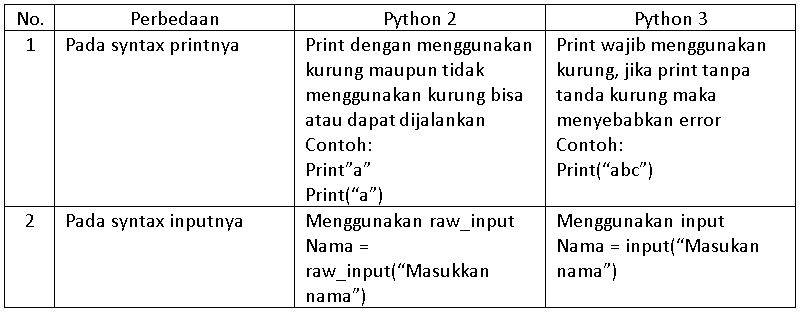
\includegraphics[scale=0.7]{figures/beda}}
        \caption{Perbedaan Python 2 dan Python 3}
		\label{beda}
\end{figure}

\subsection{Implementasi dan Penggunaan Python di Perusahaan Dunia}
\begin{enumerate}
\item Spotify 
\par
Spotify adalah suatu layanan musik streaming yang menggunakan bahasa pemrograman python untuk analisis data dan backend. Pada backend spotify berkomunikasi dengan 0MQ. 0MQ adalah suatu framework dan library open source untuk networking. Untuk analisis data tersebut, spotify menggunakan luigi, dan modul python yang sinkron dengan hadoop.
\item Google
\par 
Google menggunakan bahasa pemprograman python. Ini sudah sajak dari awal berdirinya. Dan saat ini bahasa pemprograman python merupakan salah satu bahasa pemprograman server-side resmi di google. Meskipun ada script yang ditulis untuk google menggunakan bahasa perl dan bash, maka nantinya script tersebut akan diubah ke python terlebih dahulu, karena kemudahan dalam perawatannya.
\item Industrial Light and Magic
\par 
Industrial Light and Magic ini merupakan studio special efek yang dibutuhkan untuk film star wars. Karena infrastruktur awal industrial light and magisc ini menggunakan C dan C++, maka akan lebih mudah mengintegrasikan bahasa pemprograman python ketimbang bahasa pemprograman lainnya. Dengan menggunakan bahasa pemprogramana python, industrial light and magic dengan mudah membungkus komponen software dan bisa meningkatkan aplikasi grafisnya.
\item Netflix
\par 
Netflix adalah suatu layanan pemutaran film yang dapat dilakukan oleh pengguna dimanapun dan kapanpun. Pada netfilx bahasa pemprograman yang digunakan adalah python, bahasa pemprograman ini digunakan pada Central Alert Gateway yang akan me-reroute alert dan mengirimkannya pada individu yang akan melihatnya serta juga  dapat secara otomatis reboot atau menghentikan proses yang dianggap bermasalah. Selain itu python juga digunakan untuk menelusuri riwayat dan perubahan pengaturan keamanan.
\item Instagram 
\par 
Instagram adalah suatu aplikasi mobile berbasis IOS, android dan windows phone, dimana pengguna dapat berbagi foto dan video melalui instagram ini. Pada instagram ini menggunakan bahasa pemprograman python dalam task queuennya atau fitur dimana setiap pengguna dapat berbagi foto atau video ke beberapa social network lainnya seperti facebook, twitter, dan lain-lainnya.

\end{enumerate}
\section{Instalasi}
\subsection{Instalasi Anaconda}
\par
	Sebelum \textit{menginstall} \textit{Anaconda Python} hal pertama yang harus diperhatikan yaitu versi dari Sistem Operasi yang digunakan, misalnya \textit{Windows} versi 32bit atau 64bit, jadi anda harus \textit{menginstall} \textit{Anaconda Python} sesuai dengan Sistem Operasi di \textit{windows} anda, karena jika versi \textit{windows} berbeda versi dengan \textit{Anaconda Python} dapat menyebabkan \textit{error}.\\


Langkah-langkah install anaconda.
Berikut langkah-langkah instalasi anaconda.
\begin{enumerate}
\item \textit{Download Anaconda Python} https://www.anaconda.com/distribution/
\item Buka aplikasi \textit{installer Anaconda} tersebut lalu akan muncul  gambar \textit{installer anaconda}. Kemudian klik \textit{next}
\begin{figure}[H]
        \centerline{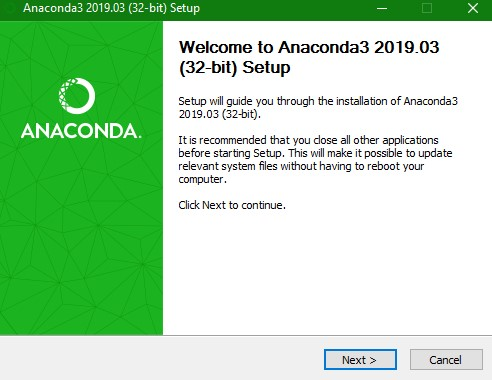
\includegraphics[scale=0.5]{figures/b}}
        \caption{Installer anaconda}
		\label{langkah1}
\end{figure}

\item Pada \textit{License agreement} klik \textit{i agree}
\begin{figure}[H]
        \centerline{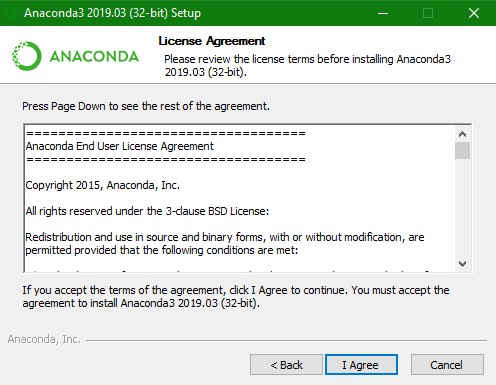
\includegraphics[scale=0.5]{figures/c}}
        \caption{License agreement}
		\label{langkah2}
\end{figure}


\item Kemudian pilih \textit{Just Me (Recomended)}kemudian klik \textit{next}
\begin{figure}[H]
        \centerline{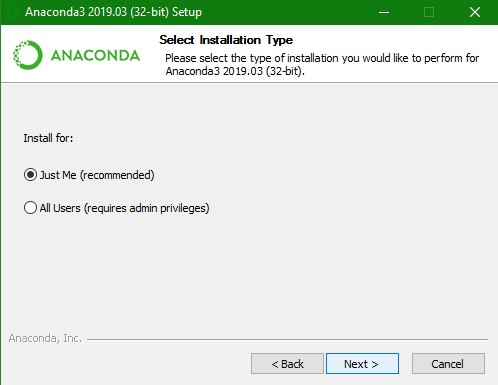
\includegraphics[scale=0.5]{figures/d}}
        \caption{\textit{Just Me(recomended)}}
		\label{langkah2}
\end{figure}


\item Kemudian pilih lokasi tempat menginstall anaconda.

\begin{figure}[H]
    \centering
    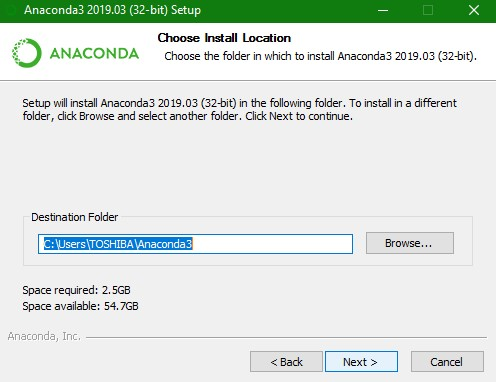
\includegraphics[scale=0.5]{figures/e}
    \caption{pilih lokasi}
    \label{Figureanaconda3}
\end{figure}


\item Kemudian centang \textit{Add anaconda to my Path envirotment variable}, agar saat menginstall selenium langsung ke path anaconda tidak ke aplikasi yang lain. Kemudian klik \textit{install}

\begin{figure}[H]
    \centering
    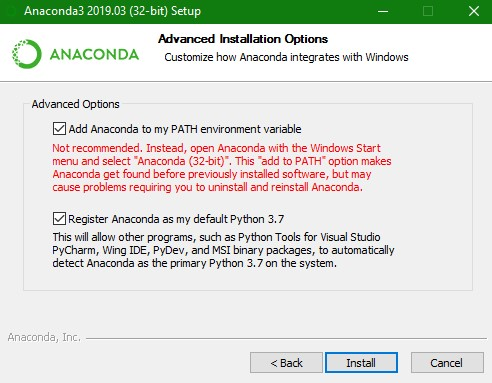
\includegraphics[scale=0.5]{figures/f}
    \caption{centang \textit{Anaconda to my Path}}
    \label{Figureanaconda4}
\end{figure}


\item Tunggu sampai proses \textit{install} selesai. Kemudian klik \textit{next}

\begin{figure}[H]
    \centering
    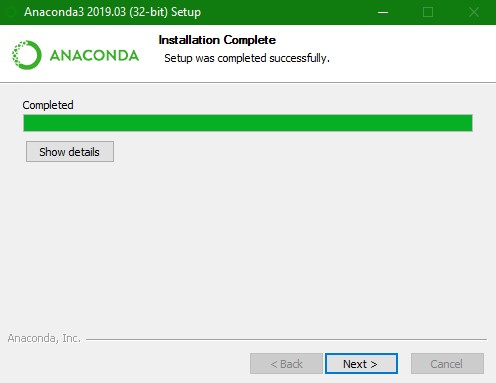
\includegraphics[scale=0.5]{figures/g}
    \caption{\textit{installation complete}}
    \label{Figureanaconda5}
\end{figure}

\item Klik \textit{next}

\begin{figure}[H]
    \centering
    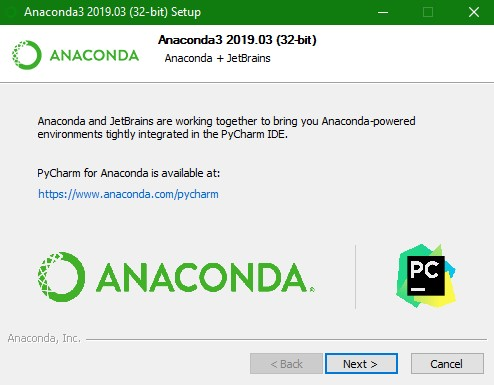
\includegraphics[scale=0.5]{figures/h}
    \caption{\textit{anaconda + jetbrains}}
    \label{Figureanaconda6}
\end{figure}

\item Jika sudah klik \textit{finish}
\begin{figure}[H]
    \centering
    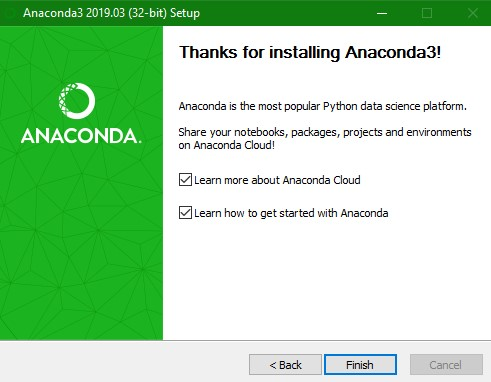
\includegraphics[scale=0.5]{figures/qz}
    \caption{\textit{thanks for install anaconda}}
    \label{Figureanaconda7}
\end{figure}


\end{enumerate}

\subsection{Setting Environment}
\begin{enumerate}
\item Buka windows explorer
\item Klik kanan pada This pc, lalu pilih properties
\begin{figure}[H]
    \centering
    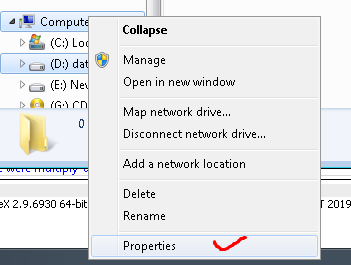
\includegraphics[scale=0.7]{figures/a1}
    \caption{\textit{Properties}}
    \label{Environment1}
\end{figure}

\item Pilih menu Advanced system settings
\begin{figure}[H]
    \centering
    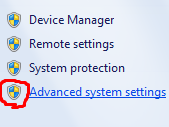
\includegraphics[scale=0.7]{figures/a2}
    \caption{\textit{Advanced system settings}}
    \label{Environment2}
\end{figure}

\item Pilih Environment Variables
\begin{figure}[H]
    \centering
    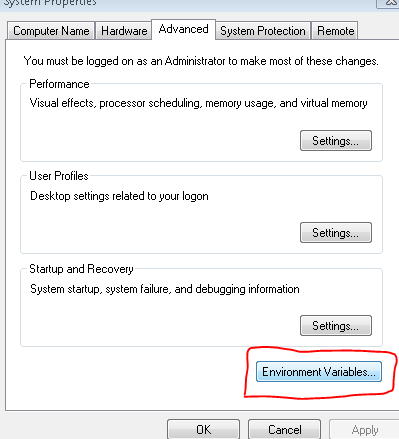
\includegraphics[scale=0.7]{figures/a3}
    \caption{\textit{Environment Variables}}
    \label{Environment3}
\end{figure}

\item Pilih Path
\begin{figure}[H]
    \centering
    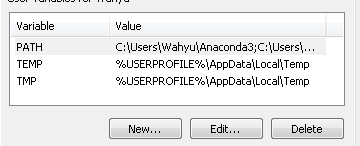
\includegraphics[scale=0.7]{figures/a4}
    \caption{\textit{Path}}
    \label{Environment4}
\end{figure}
\item lalu pilih environment variable yang ingin ditambahkan, klik OK

\end{enumerate}

\subsection{Command Line Interface/Interpreter}
\begin{enumerate}
\item Buka cmd kemudian ketik python
\item Membuat perintah untuk print, input, perkalian, dan pembagian

\begin{figure}[H]
    \centering
    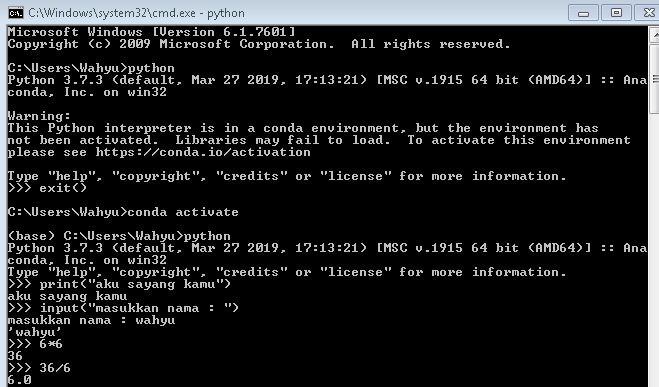
\includegraphics[scale=0.5]{figures/a5}
    \caption{\textit{CLI in Command Prompt}}
    \label{CLI}
\end{figure}
\end{enumerate}

\subsection{Instalasi pip}

\par Karena saya sudah mencoba menginstall pip dengan mengetik install -c anaconda pip tapi error saya mencoba cara lain yaitu dengan
\begin{enumerate}
\item buka browser cari get.pip
\begin{figure}[H]
    \centering
    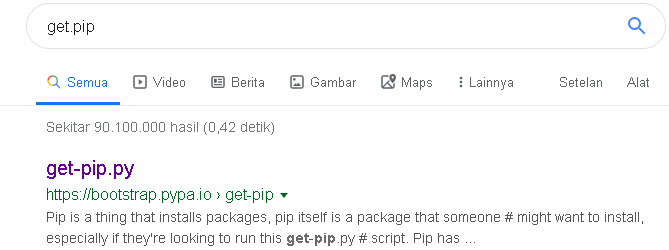
\includegraphics[scale=0.5]{figures/b1}
    \caption{\textit{get.pip}}
    \label{getpip}
\end{figure}

\item kemudian save filenya atau dengan ctrl+s save di desktop
\begin{figure}[H]
    \centering
    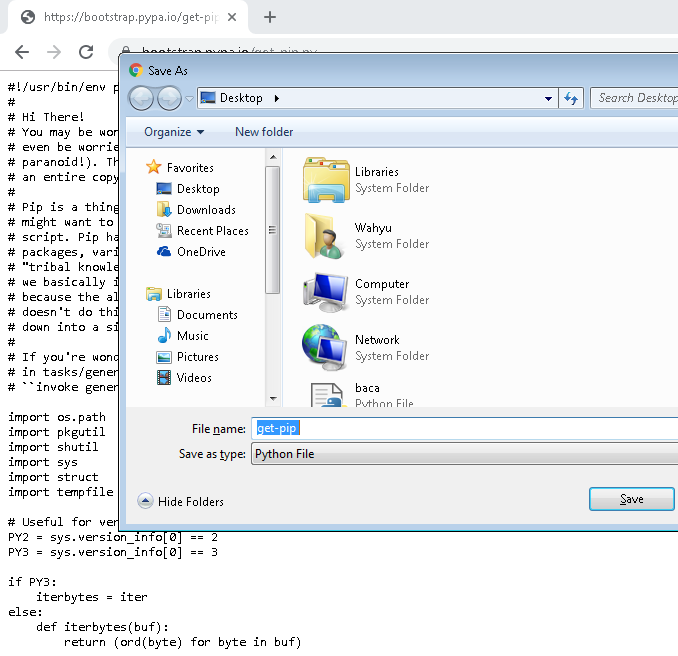
\includegraphics[scale=0.5]{figures/b3}
    \caption{\textit{save get.pip}}
    \label{getpip}
\end{figure}

\item kemudian buka cmd ketik cd desktop untuk pindah ke direktori desktop, jika sudah ketik get-pip.py dan tunggu sampai proses selesai
\begin{figure}[H]
    \centering
    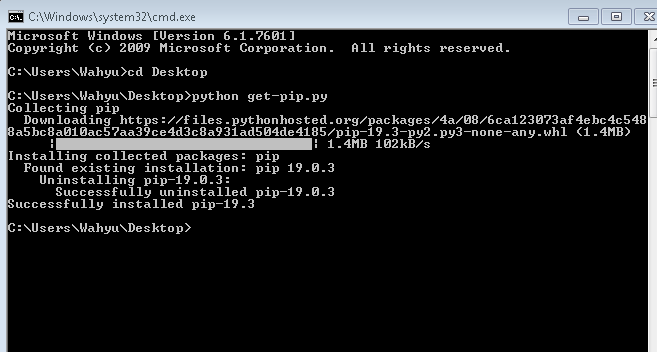
\includegraphics[scale=0.5]{figures/b4}
    \caption{\textit{python get-pip.py}}
    \label{getpip}
\end{figure}
\end{enumerate}

\subsection{Menjalankan Script Hello World di Spyder}
\begin{enumerate}
\item Buka spyder


\item ketikkan print("Hello World") kemudian run
\begin{figure}[H]
    \centering
    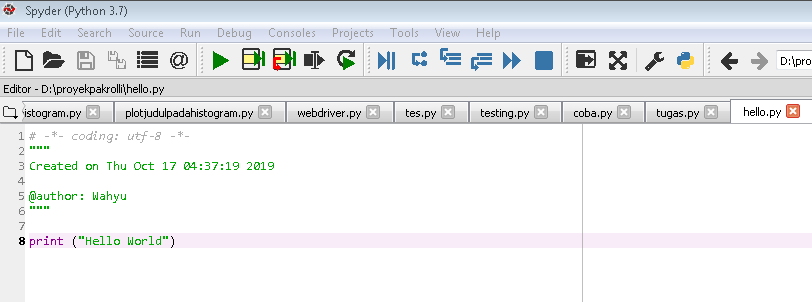
\includegraphics[scale=0.6]{figures/a8}
    \caption{\textit{Print Hello World}}
    \label{Print Hello World}
\end{figure}

\item hasilnya akan seperti ini
\begin{figure}[H]
    \centering
    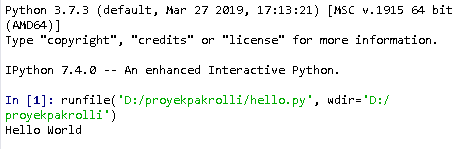
\includegraphics[scale=0.6]{figures/a9}
    \caption{\textit{Hello World}}
    \label{Hello World}
\end{figure}
\end{enumerate}

\subsection{Otomatis Login di siap.poltekpos}
Buka Spyder kemudian ketikkan script sebagai berikut.
\begin{verbatim}
from selenium.webdriver import Firefox
from selenium.webdriver.firefox.options import Options
from selenium.webdriver.common.desired_capabilities import DesiredCapabilities
from selenium.webdriver.firefox.firefox_binary import FirefoxBinary

print("Masukkan Npm Anda:")
npm = input()
print("Masukkan Password SIAP Anda:")
paswd = input('')

opsi = Options()

opsi.headless = False
binary = FirefoxBinary("C:\\Program Files\\Mozilla Firefox\\firefox.exe")
cap = DesiredCapabilities().FIREFOX
cap['marionette'] = True

browser=Firefox(executable_path='geckodriver.exe',
options=opsi,capabilities=cap,firefox_binary=binary)
browser.get('http://siap.poltekpos.ac.id/siap/besan.depan.php')

name = browser.find_element_by_name('user_name')
word = browser.find_element_by_name('user_pass')
login = browser.find_element_by_name('login')

name.send_keys(npm)
word.send_keys(paswd)
login.click()
\end{verbatim}

Kemudian save program dengan nama loginsiap.py kemudian run program atau klik f5
\begin{figure}[H]
    \centering
    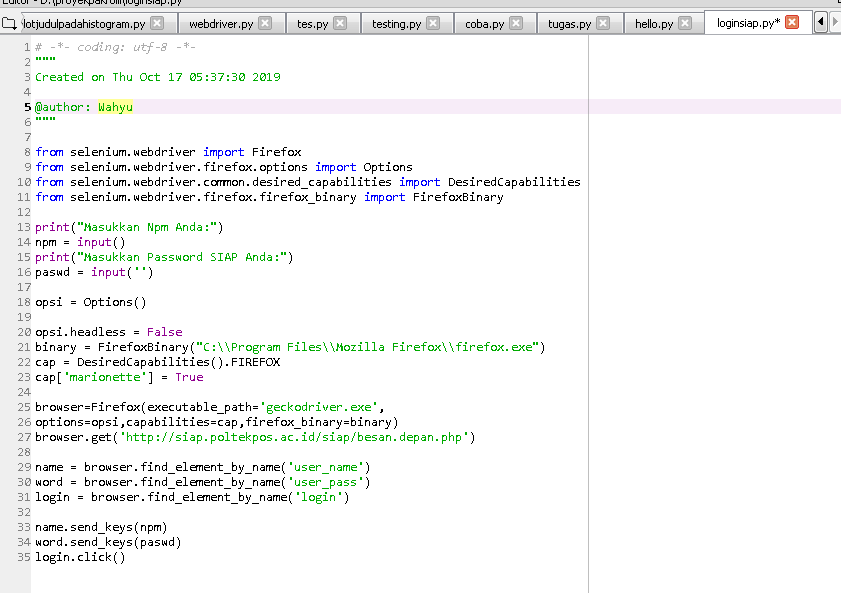
\includegraphics[scale=0.5]{figures/a10}
    \caption{\textit{Automatic Login SIAP}}
    \label{Automatic1}
\end{figure}
Setelah di run maka akan diminta untuk menginputkan NPM dan Password agar bisa login ke akun SIAP
\begin{figure}[H]
    \centering
    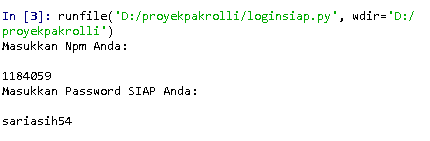
\includegraphics[scale=0.5]{figures/a11}
    \caption{\textit{Hasil Running}}
    \label{Automatic2}
\end{figure}
Program selanjutnya akan membuka mozilla firefox secara otomatis dan mengetikkan NPM serta password yang telah diinputkan oleh user dan kemudian mengklik login secara otomatis juga.
\begin{figure}[H]
    \centering
    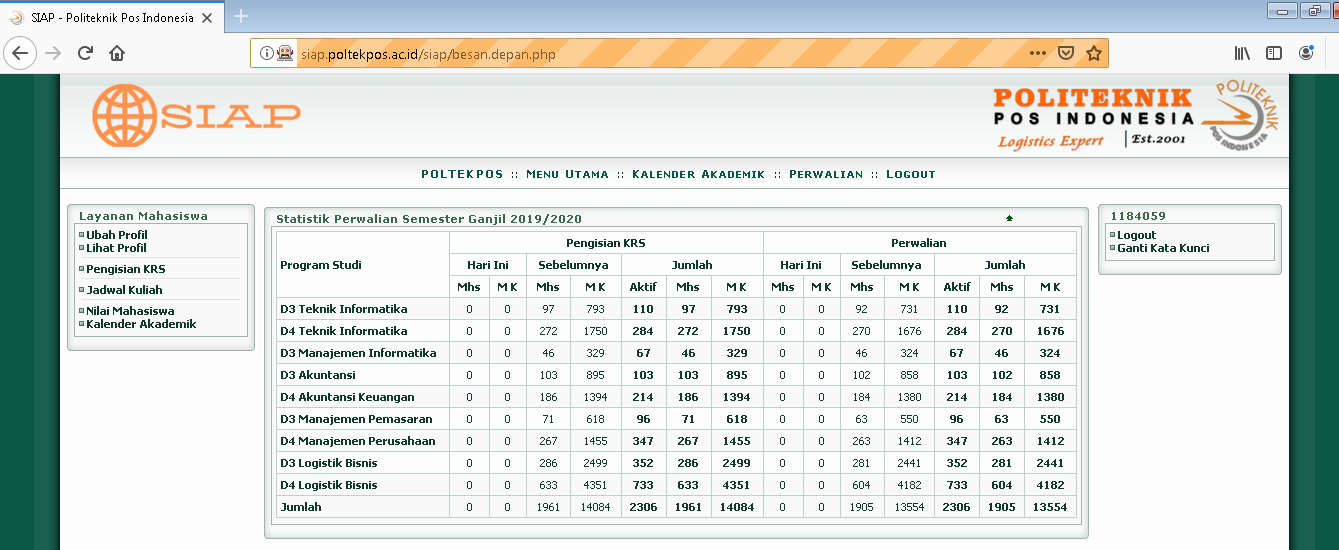
\includegraphics[scale=0.4]{figures/a12}
    \caption{\textit{Automatic Input dan Login}}
    \label{Automatic3}
\end{figure}


\subsection{Pemakaian Variable Explorer}
Variable explorer akan secara otomatis terisi ketika kita membuat suatu variable, pada variable explorer kita bisa melihat nama variable, tipe data, size dari variable tersebut.
\begin{figure}[H]
    \centering
    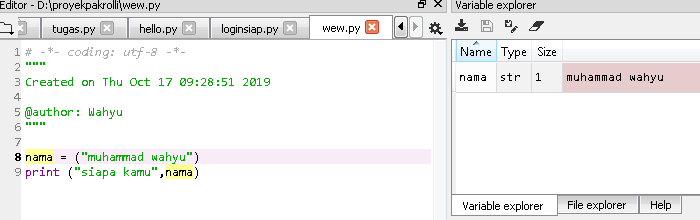
\includegraphics[scale=0.4]{figures/b5}
    \caption{\textit{Variable Explorer}}
    \label{Variable Explorer}
\end{figure}

\section{Indentasi}
\subsection{Penjelasan Indentasi}
Identasi adalah bagian dari suatu paragraf yang menjorok kedalam pada baris tiap paragraf. Mengatur indentasi dengan cara menggunakan tab atau spasi. Identasi digunakan oleh bahasa pemrograman python sebagai pengganti briket ({}) untuk membuka dan menutup suatu fungsi. Error indentasi dapat terjadi jika syntax tidak menggunakan tab atau space.


\subsection{Jenis-Jenis Error Indentasi}

\begin{figure}[H]
    \centering
    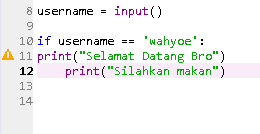
\includegraphics[scale=0.5]{figures/b6}
    \caption{\textit{Indentasi}}
    \label{Indentasi}
\end{figure}
Jika di run muncul error seperti ini.
\begin{figure}[H]
    \centering
    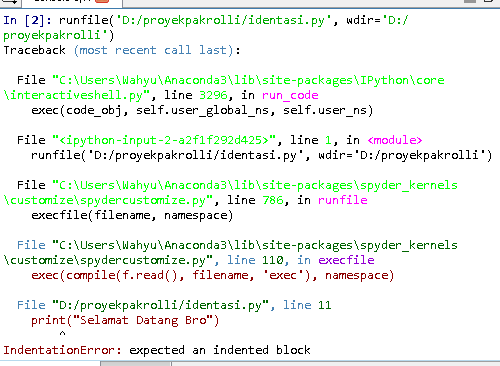
\includegraphics[scale=0.4]{figures/b7}
    \caption{\textit{Error Indentasi}}
    \label{Error Indentasi}
\end{figure}


\subsection{Cara Menangatasi Error}
Mengatasi error indentasi dapat dilakukan dengan cara menambahkan tab atau space pada line yang terdapat error.

\begin{figure}[H]
    \centering
    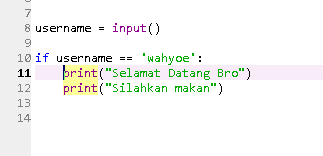
\includegraphics[scale=0.7]{figures/b8}
    \caption{\textit{Syntax yang Telah Diperbaiki}}
    \label{Syntax Error}
\end{figure}